\graphicspath{{images/}}

\section{Results}
\label{sec:results}

% \subsection{\thesubsection~Guessing}
% \end{multicols}
% \graphicspath{{images/guessing/}}
% \begin{Figure}
%   \centering
%   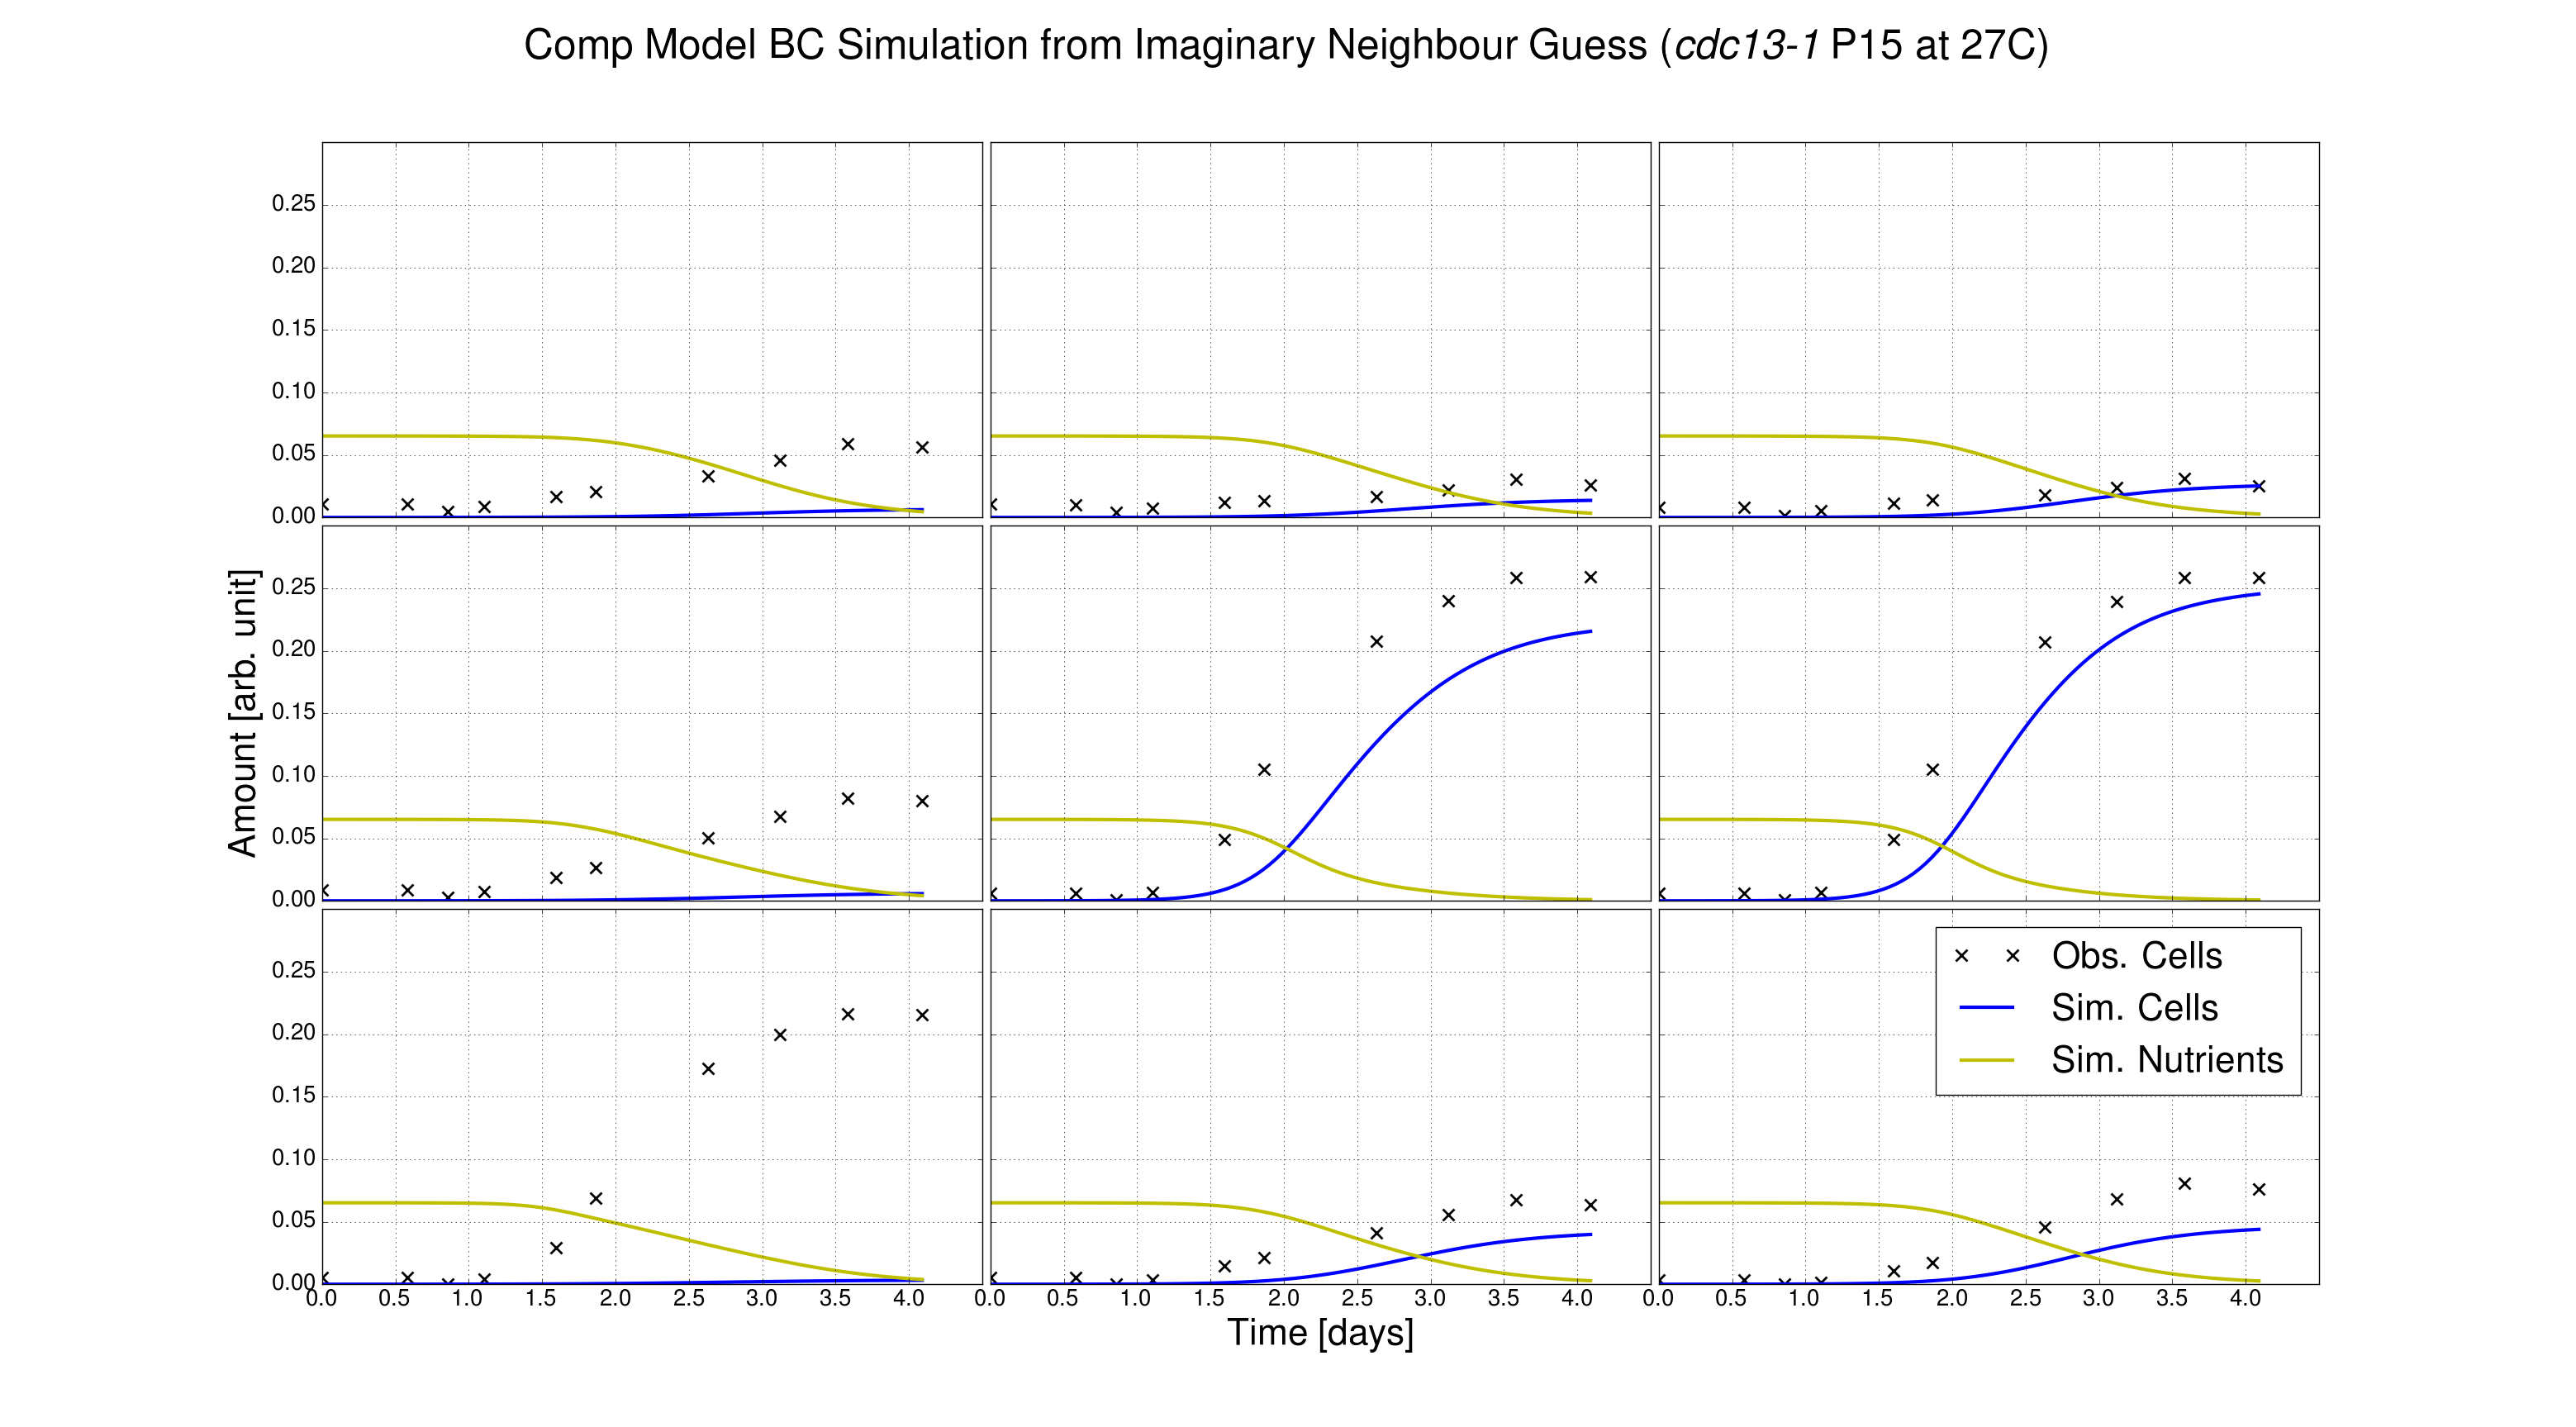
\includegraphics[width=\linewidth]{final/P15_R5_C18_guess_sim}
%   \captionof{figure}{\textbf{Competition model simulation using
%       parameters from imaginary neighbour guessing.} Shows a 3x3 zone
%     with top-left coordinate (5, 18) from P15 with background
%     \textit{cdc13-1} at 27\(^{\circ}C\).}
%   \label{fig:imag_neigh_guess_sim}
% \end{Figure}
% \begin{multicols}{2}

% Scripts were run with combinations of the following values.
% cellratios = np.logspace(-3, -5, num=5)
% fittype = ["imagneigh", "logeq"]
% zerokn = [True, False]

% Each script looped through the following array of b values which were
% supplied to the initial guesser and used at the plate level.

% for b-guess in [35, 40, 45, 50, 55, 60, 65, 70, 75, 80, 95, 100, 150]:

\subsection{Model comparison using P15}
\label{sec:P15_fit}
\subsubsection{Quality of fit}

I compared the competition and logistic models by fitting both to P15
(data described in Section~\ref{sec:P15_description}). For the
competition model, I used five values of \(C(0)\) over the range
\(N(0)\times\)10\(^{-5} < C(0) < N(0)\times\)10\(^{-3}\) to make
initial parameter guesses as described in
Section~\ref{sec:initial_guess}. This generated 70 initial parameter
sets which I used in 70 separate fits. Cell density estimates fit data
closely (Figure~\ref{fig:comp_fit_plate}).
% Timecourses for the best fit are shown in
% Figure~\ref{fig:comp_fit_plate}. Cell density estimates fit data
% closely.
A high nutrient diffusion constant, \(k\), is estimated, such that
nutrients diffuse readily and nutrient timecourses are similar across
local areas of the plate. Estimated parameters for the two closest
fits are show in Table~\ref{tab:P15_best_fit_params}. \(N_{I}(0)\) and
\(N_{E}(0)\) agree better than \(C(0)\) and \(k\). It appears that the
gradient method is not finding a global minimum. However, \(b_{i}\)
estimates are correlated with Spearman's rank correlation coefficient,
\(\rho_{S} = 0.989\), and have average mean absolute deviation,
\(MAD = 1.56\). The mean value of \(b\) for the best fit is 44.4, so
agreement between \(b_{i}\) are good. This is important because \(b\)
is to be used as a fitness estimate to compare with the logistic
model.
\begin{center}
  \captionof{table}{\textbf{Estimated parameters for the two best
      competition model fits to P15.} Spearman's rank correlation
    coefficient (\(\rho_{S}\)) between \(b\) estimates is 0.989. Mean
    absolute deviation (MAD) between \(b\) estimates is 1.56. Mean
    \(b\) for the best fit is 44.4. Obj.~is the total objective
    function value for internal cultures (smaller values are better).}
  \begin{tabular}{l l l l l l}
    \hline
    Fit     & \(C(0)\)                    & \(N_{I}(0)\) & \(N_{E}(0)\) & \(k\) & Obj.\\
    \hline
    1st     & 9.1\(\times\)10\(^{-5}\)    & 0.064      & 0.090       & 6.7  & 0.194 \\
    2nd     & 13.9\(\times\)10\(^{-5}\)   & 0.062      & 0.097       & 8.3  & 0.196 \\
    \hline
  \end{tabular}
  \label{tab:P15_best_fit_params}
\end{center}
% For all comparisons between the top four fits, \(\rho_{S}\) ranges
% from 0.922 to 0.995 and \(b\) MAD ranges from 1.56 to 6.90. I
% discarded the 5th best fit, which has less agreement, because, unlike
% the other fits, it estimated \(N_{I}(0)\) > \(N_{E}(0)\). When
% comparing this outlier with the top four fits, \(\rho_{S}\) is above
% 0.930, but \(b_{i}\) are more affected, with a maximum MAD of
% 13.29. Despite not finding a global minimum, the best competition
% model estimates of \(b_{i}\) agree well enough with each to allow
% meaningful comparison with logistic model parameter estimates.

The boxed 3x3 zone in Figure~\ref{fig:comp_fit_plate} is replotted in
Figure~\ref{fig:P15_zone_fit} with fits of the competition model
(solid blue and yellow), initial guess (dashed blue and yellow), and
logistic model (solid red). The zone contains more fast growing
cultures than is typical for the plate, so competition effects might
be greater than average.
% The logistic model was fit using the QFA R package \citep{qfa2016}.
The fit of the initial guess is typical for the plate: timecourses for
some cultures, such as the bottom-left, are poor. Nevertheless, the
guess fulfils its purpose by allowing a good fit of the competition
model to be made. Objective function values for the logistic and
competition model are similar for most cultures in the zone. For the
centre and centre-right fast growing cultures, however, the
competition model has much lower objective function values and fits
are closer. The total objective function value for the zone is lower
for the competition model: 44.06 vs 68.38 (values scaled by
\(10^{4}\)). This is not typical for the plate; objective function
values are on average slightly better for the logistic model (see
Table~\ref{tab:P15_obj_fun}). Recall that only internal objective
function values are used to assess the fit. Overall, the competition
model performed well considering that it used far fewer parameters
(387 vs 1152).

\graphicspath{{images/p15_fits/}}
\begin{Figure}
  \centering
  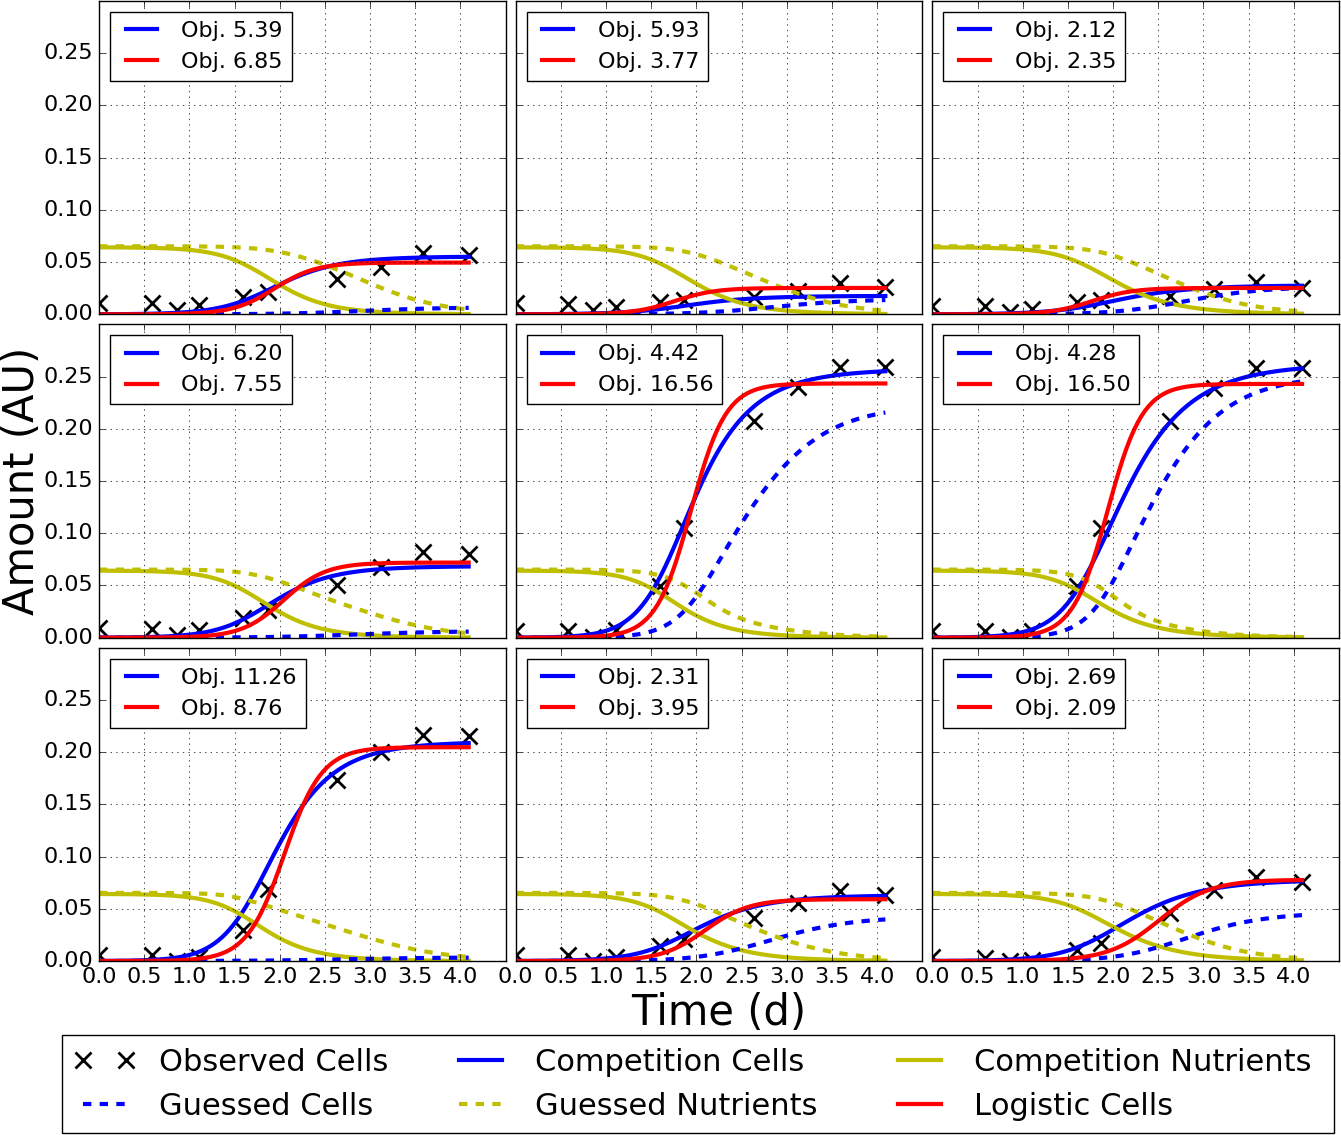
\includegraphics[width=\linewidth]{final/zone_r5_c18_with_obj_fun_2}
  \captionof{figure}{\textbf{A 3x3 zone of P15 showing fits of the
      competition and logistic models}. The zone has top-left
    coordinates (5, 18) and is boxed in red in
    Figure~\ref{fig:comp_fit_plate}. This is a zoom on a whole plate
    fit, not just a fit to the zone. Fits are for the competition
    model (blue and yellow solid); logistic model (solid red), and
    initial guess (blue and yellow dashed). Objective function values
    (Obj.), scaled by \(10^{4}\), are displayed for each culture
    (smaller values are better).}
  \label{fig:P15_zone_fit}
\end{Figure}

% Make landscape and take a whole page.
\end{multicols}
\begin{landscape}
\graphicspath{{images/comp_fit/}}
\begin{Figure}
  \centering
  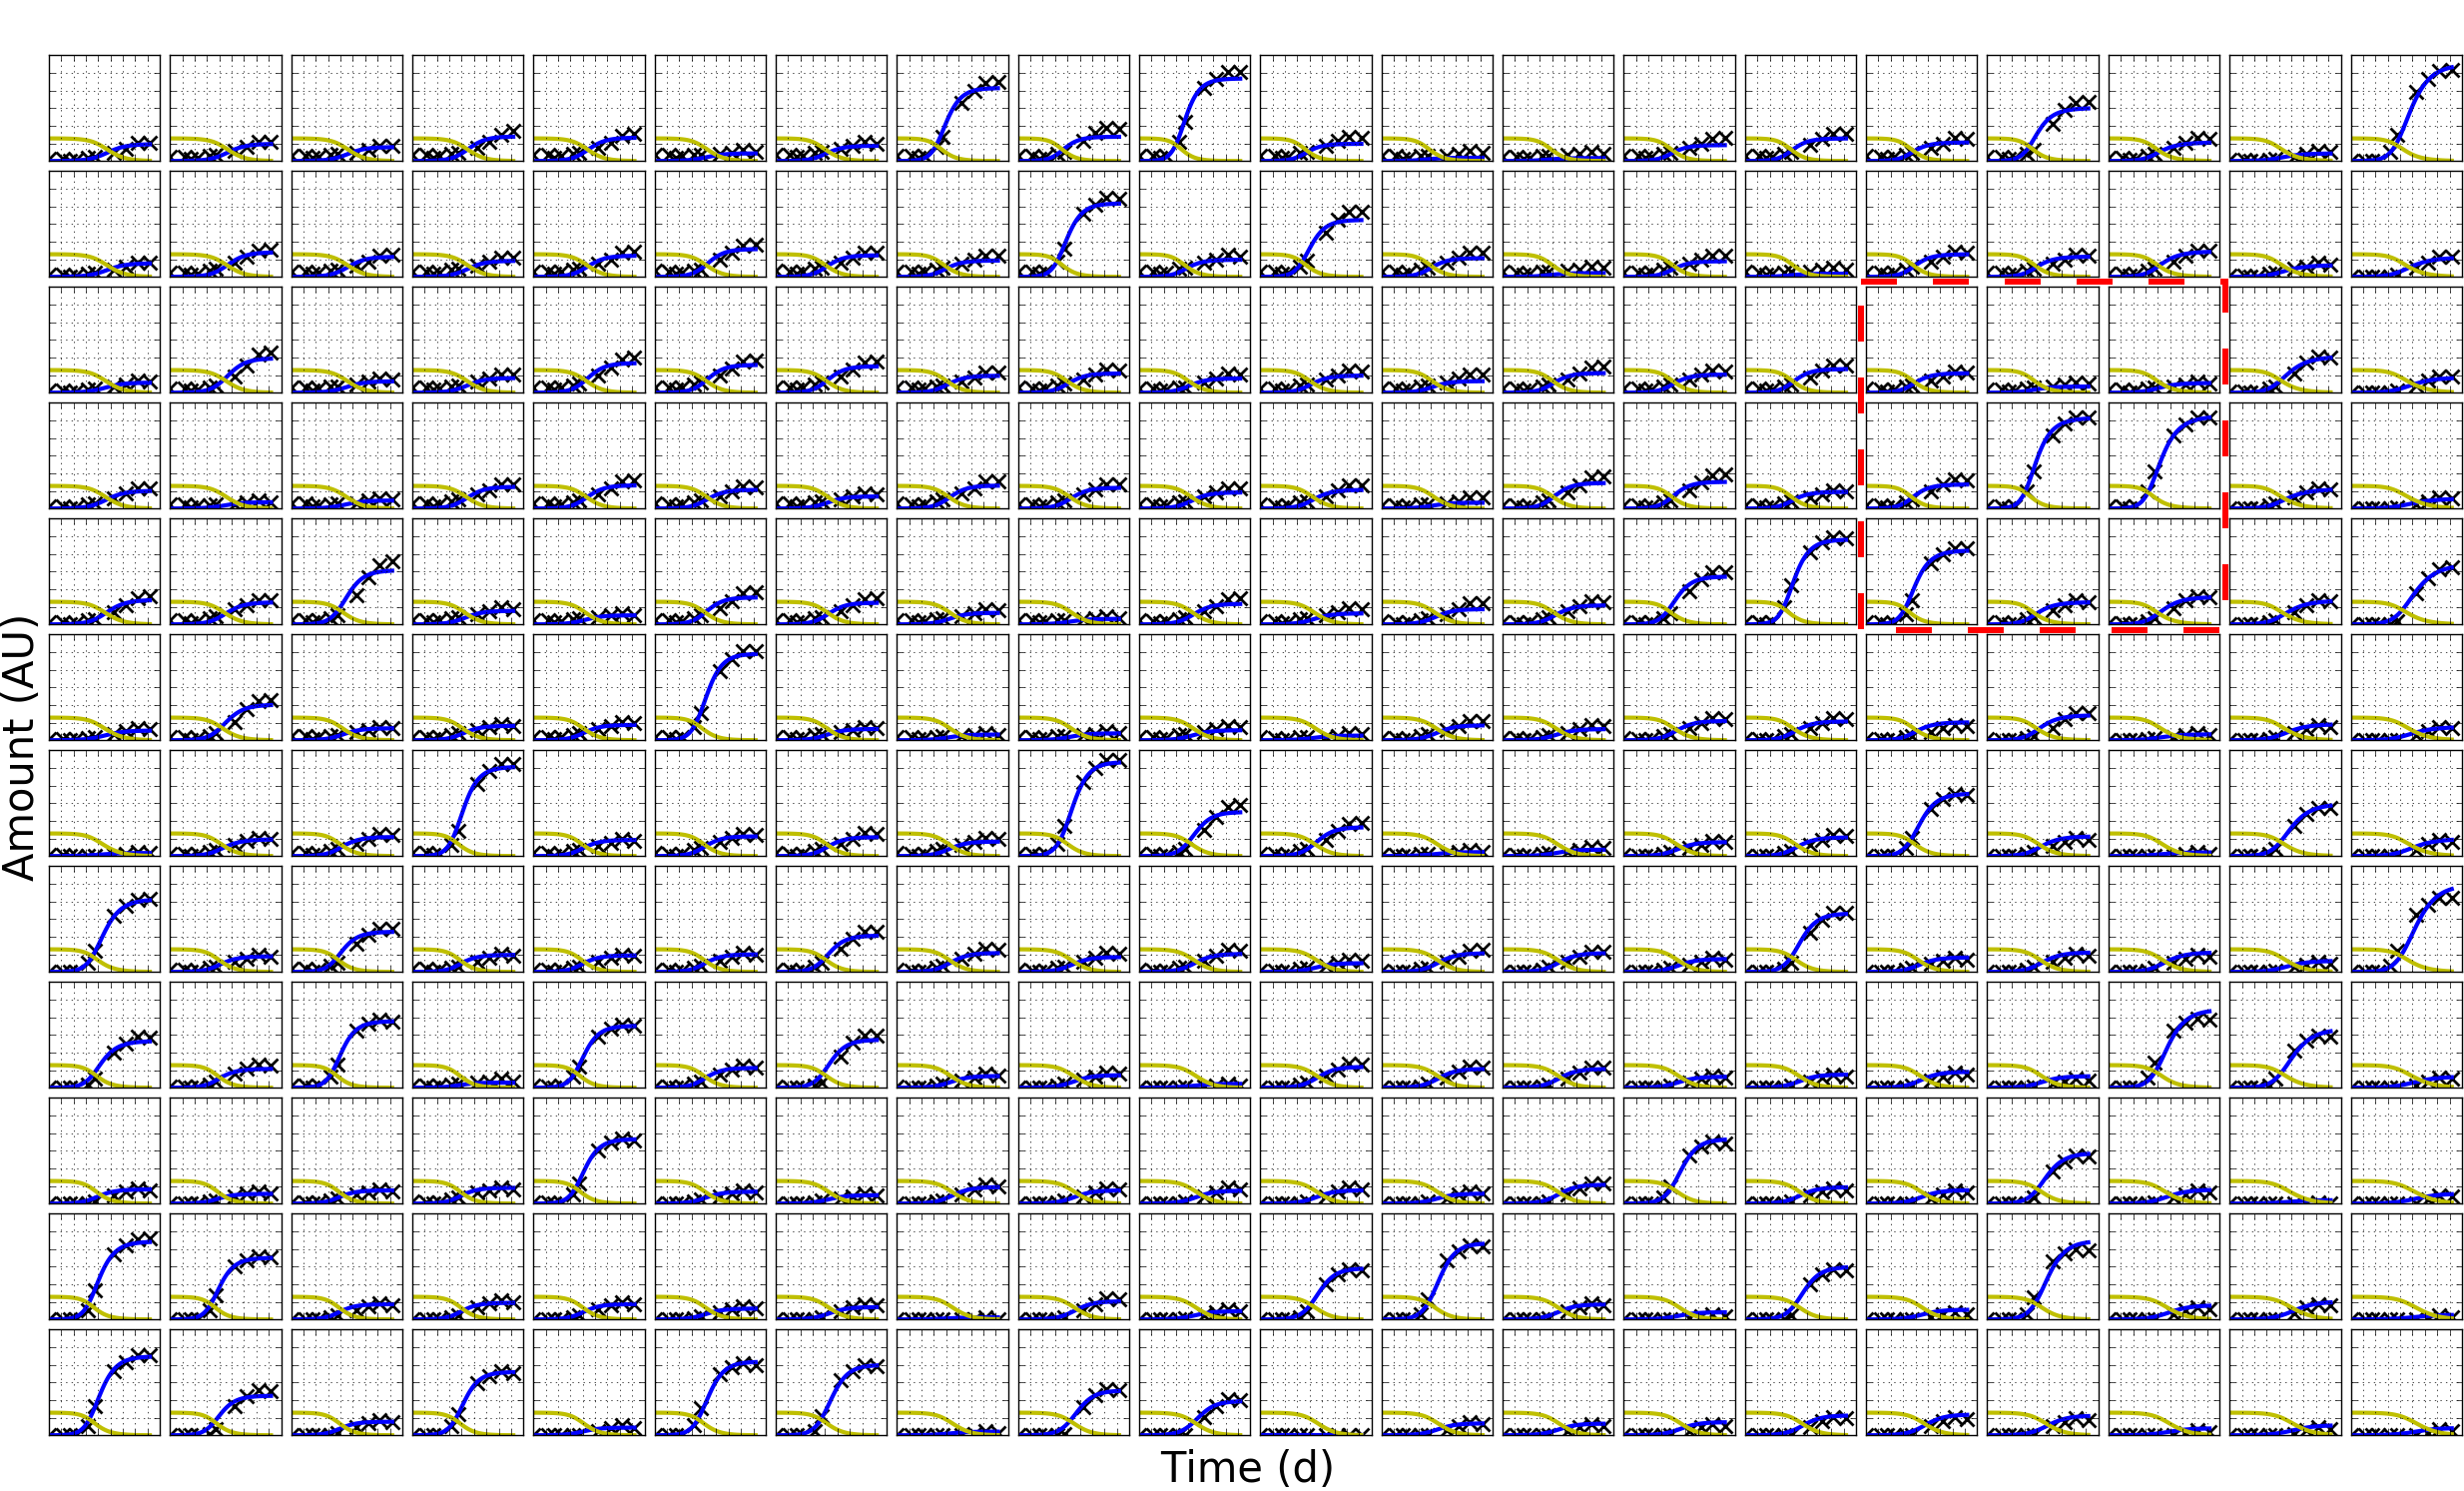
\includegraphics[width=\linewidth]{full_plate/final/P15_12x20_2}
  \captionof{figure}{\textbf{Fit of the competition model to P15.}
    Data are for a 16x24 format plate (P15) with background mutation
    \textit{cdc13-1} incubated at 27\(^{\circ}C\). The plate contains
    6 repeats of 50 genetic strains arranged randomly across internal
    cultures. The outer two rows and columns have been removed from
    the image to better fit the page. Model output for state variable,
    cell population size (blue curve), is fit to observed data (black
    crosses). Model predictions for unobserved variable (nutrient
    amount) are also plotted (yellow). The boxed zone is plotted at a
    larger size in Figure~\ref{fig:P15_zone_fit}.}
  \label{fig:comp_fit_plate}
\end{Figure}
\end{landscape}
\begin{multicols}{2}

\begin{center}
  \captionof{table}{\textbf{Objective function values for competition
      and logistic model fits to P15.} ``Internal'' is the total
    objective function value for cultures not at an edge and is used
    to select the best fit. ``All'' is the total objective function
    value for all cultures on the plate. Smaller values are better.}
  \begin{tabular}{l l l}
    \hline
    Cultures     & Competition & Logistic \\
    \hline
    Internal     & 0.194    & 0.155\\
    All          & 0.465    & 0.345\\
    \hline
  \end{tabular}
  \label{tab:P15_obj_fun}
\end{center}

\subsubsection{Correlation of fitness estimates}
\label{sec:correlation}

To compare fitness estimates between models, I converted competition
model \(b\) to logistic model \(r\) using (\ref{eq:conversion}).
% I took the median \(r\) for each deletion for both the competition
% and logistic model. I took the median, rather than mean, to reduce
% the effect of outliers that may results from cross-contamination of
% strains or inoculation of dead cells.
I plotted correlation between \(r\) estimates for each culture (black)
and between median \(r\) estimates for each deletion (red)
(Figure~\ref{fig:P15_correlations}).
% competiton model r is corrected to independent conditions.
For individual cultures, the competition model distribution is
unimodal, the logistic model distribution bimodal with minimum at
\(r \approx 4\). There are two distinct correlated groups: the first
with lower \(r\) and gradient close to one, the second with higher
\(r\) and a steeper gradient. Cultures from the middle of the
competition model distribution, but not the tails, are split between
groups. Competition model \(r\) was lower than logistic model \(r\)
for almost all cultures. There are several outlying cultures (black)
caused by failures of heuristic checks from the QFA R package. For the
eight outliers on the left axis, checks set \(r\) = 0. The two
outliers with very high logistic \(r\) are the deletions
\textit{rad50\(\Delta\)} and \textit{est1\(\Delta\)}. They have
escaped heuristic checks and exhibit a confounding effect between
\(r\) and \(K\).

\graphicspath{{images/p15_correlations/}}
\begin{Figure}
  \centering
  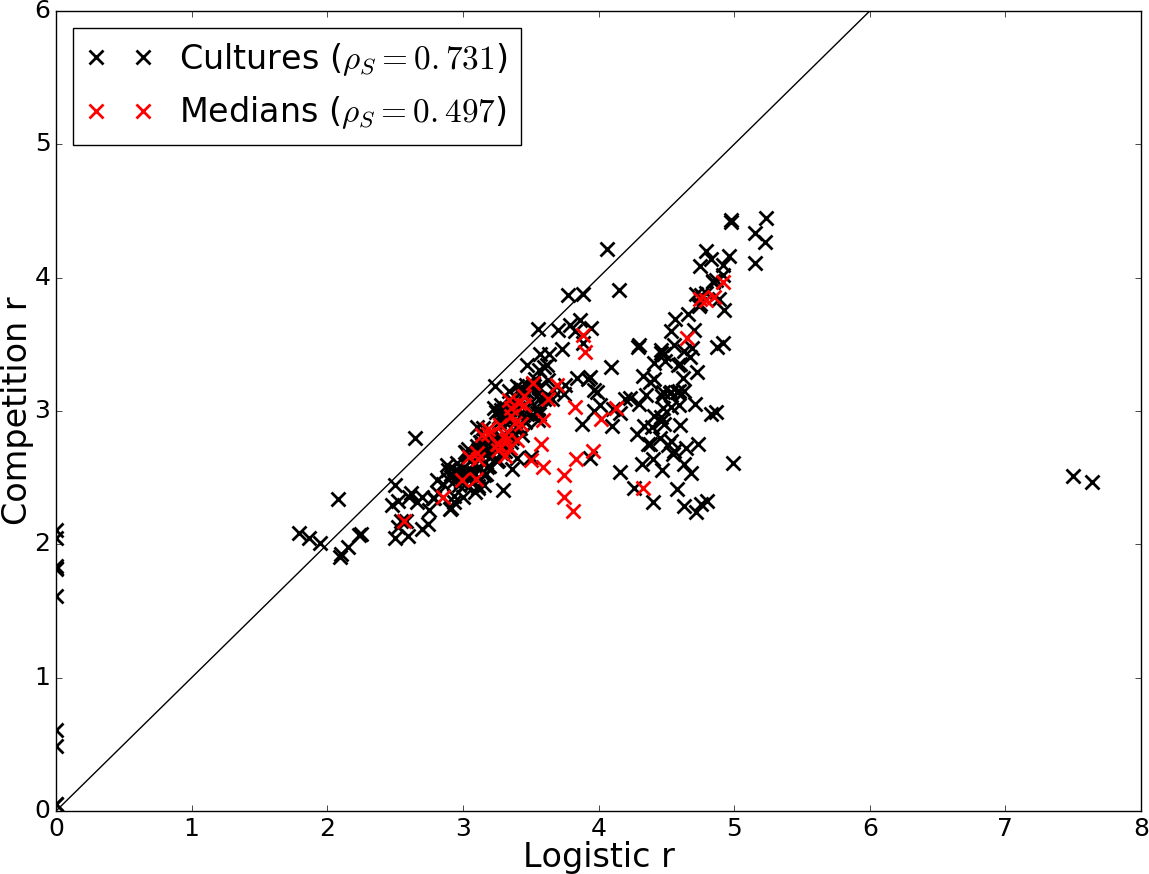
\includegraphics[width=\linewidth]{final/r_correlations_median_spearmans_trimmed_2}
  \captionof{figure}{\textbf{Correlation between logistic and
      competition model r for P15}. Correlations are between estimates
    for each culture (black) and between median estimates (six
    repeats) for each deletion (red). Spearman's rank correlation
    coefficient, \(\rho_{s}\), is displayed for each distribution. The
    line y = x is also plotted.}
  \label{fig:P15_correlations}
\end{Figure}

In the distribution of medians (red), most deletions fall inside the
denser group of cultures with lower logistic \(r\). Several deletions,
with high competition model \(r\), fall inside the second group
(top-right). A significant number of deletions, however, lie in the
region between the two groups, meaning that repeats of these cultures
are split between groups. This may also be true for other
deletions. Correlation, measured by Spearman's rank correlation
coefficient, \(\rho_{S}\), is lower between medians (0.497) than
between cultures (0.731).

\subsubsection{Comparison of fitness rankings}

I compared between models the ranking of strains by median fitness
(Figure~\ref{fig:comp_vs_log_ranking}). Rankings of competition model
\(b\), \(r\), and \(MDR\) are equivalent (see
Section~\ref{sec:parameter_conversion}), so I compared \(b\) directly
with logistic model \(r\) and \(MDR\). The latter agree in the order
of all but two deletions: \textit{rad50\(\Delta\)} and
\textit{est1\(\Delta\)}. These deletions each have an explained
outlier with unrealistically high \(r\) and low \(K\)
(Section~\ref{sec:correlation}). This appears to have been corrected
for when \(MDR\) was calculated (\ref{eq:MDR_MDP}a), and \(MDR\) rank
agrees much better with the competition model. Spearman's Rho is
therefore higher between competition \(b\) and logistic \(MDR\)
(0.635) than between competition \(b\) and logistic \(r\)
(0.497). Between models, there is good agreement in extreme positions,
but middle positions are almost inverted. The positions of the neutral
deletion, \textit{his3\(\Delta\)} (bold), disagree by 13 places.

\graphicspath{{images/rank/}}
\begin{Figure}
  \centering
  \includegraphics[width=\linewidth]{final/median_ranks_comp_b_log_r_MDR}
  \captionof{figure}{\textbf{Comparison of competition and logistic
      fitness rankings for P15.} Deletions, each with six repeats, are
    ranked according to median fitness, with the fittest strain at the
    top. Spearman's Rho is 0.497 between competition \(b\) and
    logistic \(r\), and 0.635 between competition \(b\) and logistic
    \(MDR\). \textbf{\textit{his3\(\Delta\)}} is a neutral deletion
    with 14 repeats.}
  \label{fig:comp_vs_log_ranking}
\end{Figure}

% \graphicspath{{images/rank/}}
% \begin{Figure}
%   \centering
%   \includegraphics[width=\linewidth]{final/comp_b_log_r_trimmed}
%   \captionof{figure}{\textbf{Comparison of \(\bm{r}\) ranking for fits
%       of the competition and logistic model to P15.} Fitnesses of
%     genetic strains are ranked most to least fit from top to
%     bottom. Competition model \(r\) was converted from \(b\), \(N_0\),
%     and \(C_0\) from the best competition model estimate. Logistic
%     \(r\) and \(MDR\) were taken from logistic model fits using the
%     QFA R package which makes heuristic checks for slow growing
%     cultures.}
%   \label{fig:comp_vs_log_ranking2}
% \end{Figure}

% Complicated correlation coefficient table
% \columnbreak
% \begin{center}
%   \captionof{table}{\textbf{Correlation coefficients between logistic
%       and competition model estimates of parameters for P15.} Pearson
%     correlation coefficient \(\rho\) and Spearman rank correlation
%     coefficient \(r_{s}\) are shown. Correlation coefficients compare
%     between logistic and competition model estimates for both \(r\)
%     and \(MDR\). Correlations are shown between estimates for each
%     culture and between median and mean estimates for each deletion.}
% \begin{tabular}{ |c|c|c|c|c| } \cline{2-5}
% \multicolumn{1}{c|}{} & \multicolumn{2}{c|}{\(r\)} & \multicolumn{2}{c|}{\(MDR\)}\\ \hline
% \multicolumn{1}{|c|}{Estimates} & \(\rho\) & \(r_{s}\) & \(\rho\) & \(r_{s}\)\\ \hline
% Culture & 0.712 & 0.731 & 0.752 & 0.754\\
% Median & 0.708 & 0.497 & 0.791 & 0.635\\
% Mean   & 0.763 & 0.594 & 0.885 & 0.732\\ \hline
% \end{tabular}
% \end{center}

% Just a fit of a zone
% \end{multicols}
% \graphicspath{{images/comp_fit/}}
% \begin{Figure}
%   \centering
%   \includegraphics[width=\linewidth]{final/P15_guess_and_fit_r5_c18}
%   \captionof{figure}{\textbf{A zone of a fit of the competition model
%       to P15 and initial guess}. The guess was made using the
%     imaginary neighbour model fit to individual cultures. Top-left
%     coordinates from Figure~\ref{fig:comp_fit_plate} (5, 18).}
%   \label{fig:comp_fit_zone_old}
% \end{Figure}
% \begin{multicols}{2}


% \subsection{\thesubsection~Agreement of b rankings}

%   text Some text Some text Some text Some text Some text Some text
%   Some text Some text Some text Some text.
% \graphicspath{{images/rank/}}
% \begin{Figure}
%   \centering
%   \includegraphics[width=\linewidth]{top_two_comp_p15_correlations_trimmed}
%   \captionof{figure}{\textbf{Comparison of \(\bm{b}\) ranking for the
%       best five competition model fits to P15.} Ranking is calculated
%     from the mean \(b\) estimate from the six repeats or each strain.}
%   \label{fig:comp_b_ranking}
% \end{Figure}

\newpage

\subsubsection{Precision of fitness estimates}
\label{sec:cross_plate_validation}

\end{multicols}
\graphicspath{{images/COV/}}
\begin{Figure}
  \centering
  \includegraphics[width=\linewidth]{final/comp_b_log_r_median_rank_his3_bold}
  \captionof{figure}{\textbf{Coefficient of variation (COV) in P15
      fitness estimates.} Shown for each deletion are COVs in
    estimates of competition model \(b\) (blue) and logistic model
    \(r\) (red). COV in competition model \(b\) and \(r\) are
    equivalent so comparison is direct. Deletions are ordered left to
    right from highest to lowest \(b\) estimate. Each deletion has 6
    repeats, except for the neutral deletion
    \textbf{\textit{his3\(\Delta\)}} which has 14.}
  \label{fig:COV}
\end{Figure}
\begin{multicols}{2}

% Use repeats on plate 15 (6 per deletion) more (14) for HIS3 to
% calculate coefficient of variation (COV) of estimated r or MDR.

Using coefficient of variation (COV), I compared the precision of
competition and logistic model fitness estimates in repeats of each
deletion (Figure~\ref{fig:COV}). COV of competition \(b\), \(r\), and
\(MDR\) is equivalent. I chose to compare to logistic \(r\), rather
than \(MDR\), because \(r\) and \(b\) are fixed properties of a
strain, whereas \(MDR\) is dependent on initial conditions (see
Equation~\ref{eq:MDR_MDP}a). This makes the former more useful for
cross-plate comparison. Regardless, COVs for logistic \(r\) and
\(MDR\) (not shown) are very similar.
% The precision of fitness estimates is of interest both as a test of
% the model and because it affects the power to infer genetic
% interactions. If we assume that biological variation in fitness
% between repeats of the same strain is small, then the better model
% should estimate the fitness of strains more precisely, regardless of
% where they grown on the plate.
The competition model is more precise for 36 out of 50 deletions, but
less precise for the 11 fastest growing (according to \(b\) ranking)
strains. The precision of both estimates tends to decrease for slower
growing strains.
% which are more affected by noise. There are
% exceptions such as \textit{png1}\(\Delta\) which might indicate an
% error in the order of \(b\) ranking.


% Deletions in Figure~\ref{fig:COV} are arranged from left to right
% according to competition model \(b\) ranking, with the fastest growing
% deletion on the left.

%  Comparing with Figure~\ref{fig:P15_correlations}, median
% values for these deletions (red) appear in the upper right of both
% groups of cultures (black), not in the gap inbetween.

% \(b\) COV tends to be smaller than \(r\) COV at smaller values of
% \(b\), where repeats are likely to divided between the groups (as
% indicated by the positions of medians inbetween groups). The slowest
% growers tend to have greater COV for both models, which is likely due
% to the greater effect of noise on cell density estimates in repeats of
% these deletions.

\subsubsection{Evaluating the treatment of boundaries}
\label{sec:treatment_of_boundaries}

To evaluate how I treat boundaries, I again fit the competition model
to P15, this time without a separate parameter for the initial amount
of nutrients in edge cultures. Recall that edge cultures must be
included when fitting the competition model, despite being discarded
from results due to noise. The quality of fit appears similar for both
the one and two \(N(0)\) models (Figure~\ref{fig:P15_corner}); the
average objective function values for the entire plate are similar but
slightly better for the two \(N(0)\) model
(Table~\ref{tab:corner}). Surprisingly, objective function values for
edge cultures are worse for this model. Nevertheless, the fit is
improved for cultures next to an edge, and, importantly, for internal
cultures overall. The two \(N(0)\) model takes a deficit from edge
cultures to improve the overall fit.

\graphicspath{{images/corners/}}
\begin{Figure}
  \centering
  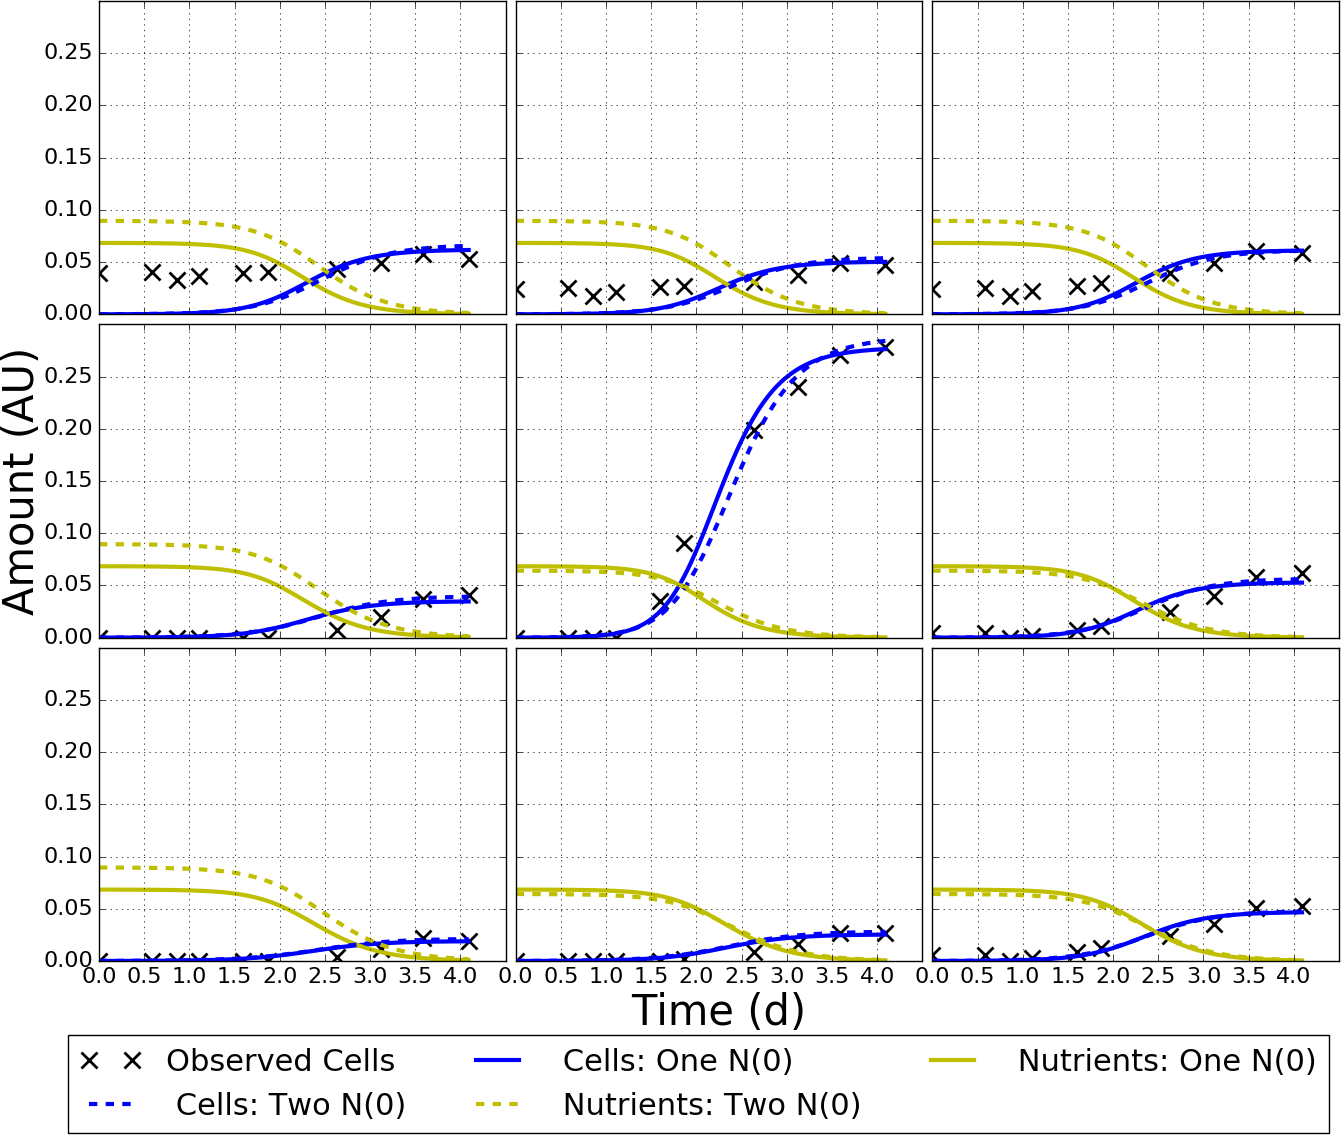
\includegraphics[width=\linewidth]{final/top_left_new_aspect_2}
  \captionof{figure}{\textbf{Fits of one and two initial nutrient
      parameter competition models to P15.} The top left corner of a
    16x24 QFA plate (P15) fit with two versions of the competition
    model: the first (solid) with a single initial nutrient amount for
    all cultures, the second (dashed) with a separate initial nutrient
    amount for edge cultures.}
  \label{fig:P15_corner}
\end{Figure}

\begin{center}
  \captionof{table}{\textbf{Average objective function values for one
      and two \(\bm{N(0)}\) parameter competition models fit to P15.}
    Lower values are better. Averages are for cultures belonging to
    the areas indicated in the column ``Cultures''. ``Next to edge''
    refers to cultures one in from the edge. ``Internal'' refers to
    all cultures but the edge.  Values have been scaled by
    \(10^{4}\).}
  \begin{tabular}{l l l}
    \hline
    Cultures     & One \(N(0)\)  & Two \(N(0)\) \\
    \hline
    Edge         & 35.9    & 36.5\\
    Next to edge & 9.54    & 7.98\\
    Internal     & 6.67    & 6.30\\
    All          & 12.4    & 12.2\\
    \hline
  \end{tabular}
  \label{tab:corner}
\end{center}

\subsection{Cross-plate validation}
\label{sec:cross_plate_val_results}

I conducted cross-plate calibration and validation of the
competition model using the Stripes and Filled plates experiment,
which is described in detail in
Section~\ref{sec:stripes_description}.
%
As for P15, I ran multiple fits to each plate (see
Section~\ref{sec:fitting_comp}). This time I used a wider range of
\(C(0)\) guesses: 10 values over
\(N(0)\times\)10\(^{-7} < C(0) < N(0)\times\)10\(^{-1}\) in
logspace. I made this decision because of the higher inoculum
densities in this experiment, and as a result of discussion with
Herrmann and Lawless, who had suggested, based on recent work, that
heterogeneity exists within individual cultures such that only a small
number of cell lines contribute significantly to final
populations. Strains in the Stripes plate are inoculated in the same
locations on the Filled plate, and empty locations on the Stripes
plate are inoculated with extra strains on the Filled plate. When
fitting, I ignored data for empty cultures which is just noise. I took
the estimated parameters for the Filled plate and simulated the
Stripes plate by setting \(b\) to zero for empty locations. The
simulated timecourses can be compared with the Stripes cell
observations to validate the competition model
(Figure~\ref{fig:stripes_validation}); if the model corrects perfectly
for differences between the plates, then simulated timecourses (blue
dashes) should fit closely to Stripes data (blue crosses). I found
that the competition model overcorrects: simulated cell densities are
higher than observations across the plate. In contrast, the logistic
model makes no adjustment between plates and systematically
underestimates observed cell densities by a similar margin.
% Good to mention here as not an important point for the discussion.
There are some issues with the experiment. For instance, the top right
culture in Figure~\ref{fig:stripes_validation} does not grow and might
have been inoculated with dead cells. Nevertheless, these mistakes are
unlikely to explain the systematic overestimation that is observed.

\end{multicols}
\graphicspath{{images/stripes/}}
\begin{Figure}
  \centering
  \includegraphics[width=\linewidth]{final/validation_r9_c10_no_nutrients}
  \captionof{figure}{\textbf{Cross-plate calibration and validation of
      the competition model.} I fit the competition model to the 16x24
    format Stripes and Filled plates
    (Section~\ref{sec:stripes_description}). The plot shows measured
    cells (crosses) and estimated cells (solid curves) from both
    plates for a 3x3 section with top left coordinates (R9, C10). I
    took the parameter estimates for the Filled plate (calibration),
    and set growth constants to zero for cultures in the empty columns
    of the Stripes plate (column two here). I then simulated using
    these parameters to produce the validation curves (dashed
    blue). If the competition model corrects for differences in growth
    between these experimental designs perfectly, the dashed blue
    curves should resemble the Stripes data (blue crosses) in columns
    one and three. The logistic model predicts no difference between
    plates.}
  \label{fig:stripes_validation}
\end{Figure}
\begin{multicols}{2}

% Estimated parameters for the best competition model fit to both plates
% are shown in Table~\ref{tab:Stripes_and_Filled_params}.
I looked more closely at estimated parameters to investigate why the
validation curves disagree with data
(Table~\ref{tab:Stripes_and_Filled_params}). All parameters disagreed
significantly between plates. Both plates used the same inoculum
density and formula of agar so I did not expect plate level parameters
to differ so much. In particular, \(k\) is much higher for the Filled
plate. Estimates of \(C(0)\) differed the least. The average \(b\)
estimate among common cultures was significantly higher for the
Stripes plate. In summary, the Stripes solution has faster growing
cultures, fewer starting nutrients, and slower diffusion.
% I should really calculate the objective function for internal
% cultures and remove the empties for the stripes plate. It is
% probably best to look at just the cultures in common. Should
% probably also normalise by cell density measurement (at each point?)
% because stripes values are all higher.
Despite these differences, both solutions fit their data with similar
closeness.
\begin{center}
  \captionof{table}{\textbf{Estimated parameter values for the best
      fit to the Stripes and Filled plates.} The mean \(b\) is taken
    only for common cultures. Spearman's rank correlation coefficient
    for \(b\) estimates between these cultures is 0.787.}
  \begin{tabular}{l l l l l l}
    \hline
    Plate     & \(C(0)\)                   & \(N_{I}(0)\) & \(N_{E}(0)\) & \(k\) & \(b\) (mean)\\
    \hline
    Stripes   & 8.3\(\times\)10\(^{-3}\)   & 0.085      & 0.096       & 1.9  & 39.5\\
    Filled    & 6.2\(\times\)10\(^{-3}\)   & 0.116      & 0.183       & 4.8  & 27.9\\
    \hline
  \end{tabular}
  \label{tab:Stripes_and_Filled_params}
\end{center}

When examining fits to the same plate, agreement between parameter
estimates is poor compared to P15; the five best fits to the Filled
plate are only consistent for initial nutrient densities
(Table~\ref{tab:Filled_best_fits}). Despite this, all solutions
overestimate growth when used to simulate the Stripes
plate. Disagreement is greater still for the Stripes plate (not
shown).
% Discusion: Further from a global minimum. Main difference is the
% higher starting cell density.
\begin{center}
  \captionof{table}{\textbf{Estimated parameter values for the best
      five competition model fits to the Filled plate.} Estimates are
    ordered by whole-plate objective function value (Obj.). Lower
    values are better. Mean Absolute Deviation (MAD) in \(b\)
    estimates is calculated against the best fit for which
    \(\mu_{b} = 27.9\). Spearman's Rho in \(b\) estimates is greater
    than 0.96 for all combinations of these fits.}
  \begin{tabular}{l l l l l l}
    \hline
    Obj.  & \(C(0)\)                  & \(N_{I}(0)\) & \(N_{E}(0)\) & \(k\) & MAD \(b\)\\
    \hline
    0.76  & 6.2\(\times\)10\(^{-3}\)   & 0.116       & 0.183    & 4.8  & -    \\
    0.85  & 5.6\(\times\)10\(^{-3}\)   & 0.119       & 0.175    & 3.1  & 0.77 \\
    0.88  & 5.0\(\times\)10\(^{-3}\)   & 0.119       & 0.175    & 2.9  & 1.65 \\
    0.93  & 15.4\(\times\)10\(^{-3}\)  & 0.114       & 0.171    & 4.7  & 11.1 \\
    0.97  & 3.2\(\times\)10\(^{-3}\)   & 0.118       & 0.179    & 3.8  & 7.80 \\
    \hline
  \end{tabular}
  \label{tab:Filled_best_fits}
\end{center}

% \graphicspath{{images/stripes/correlations/}}
% \begin{Figure}
%   \centering
%   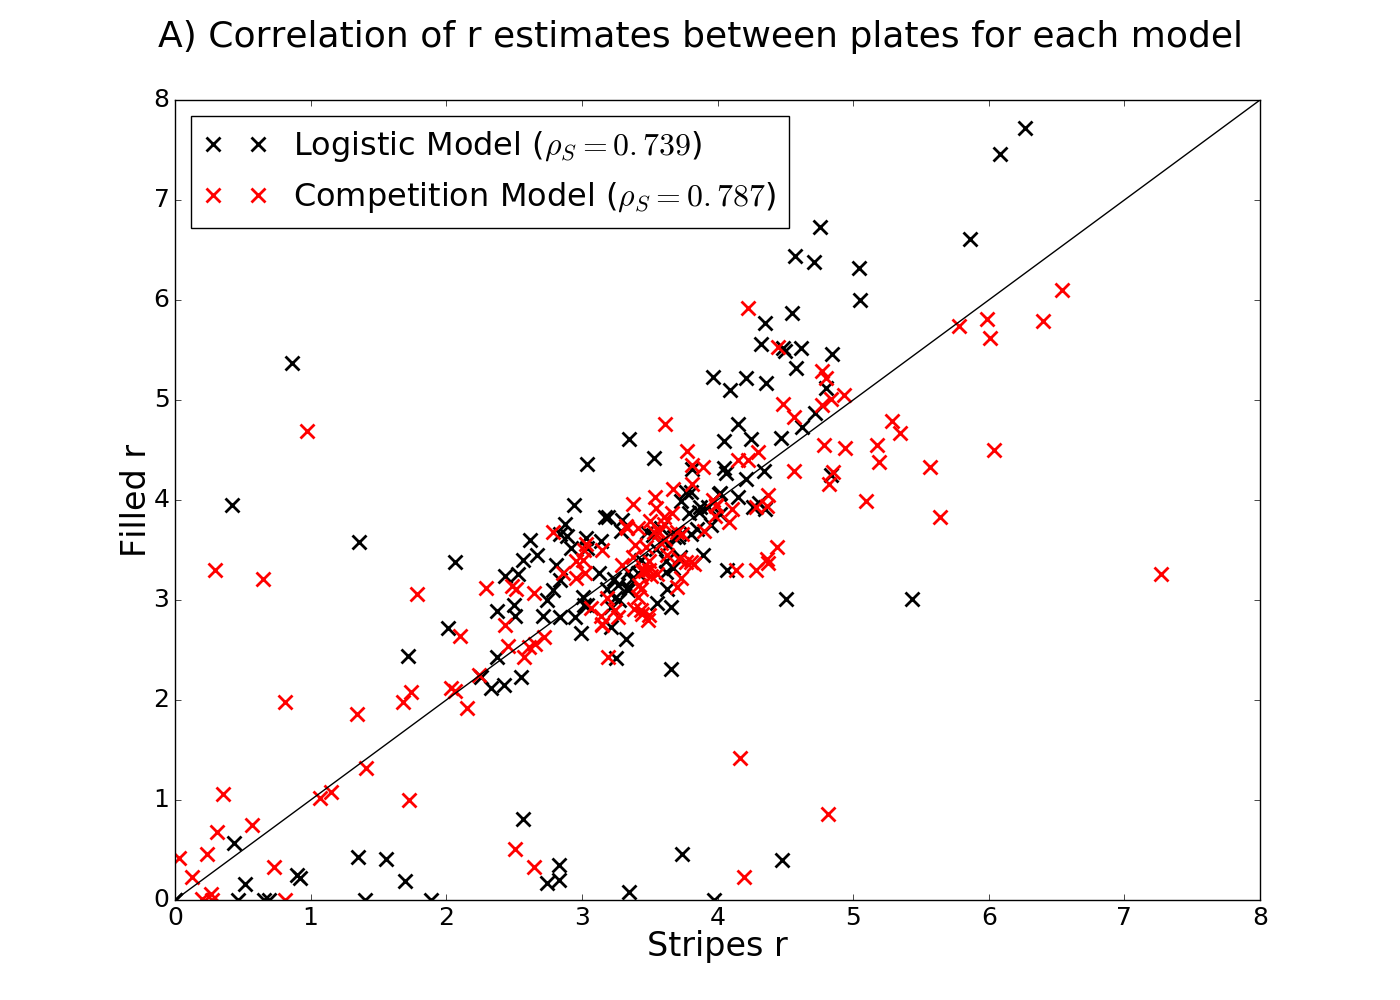
\includegraphics[width=\linewidth]{final/r_correlations_between_plates}
%   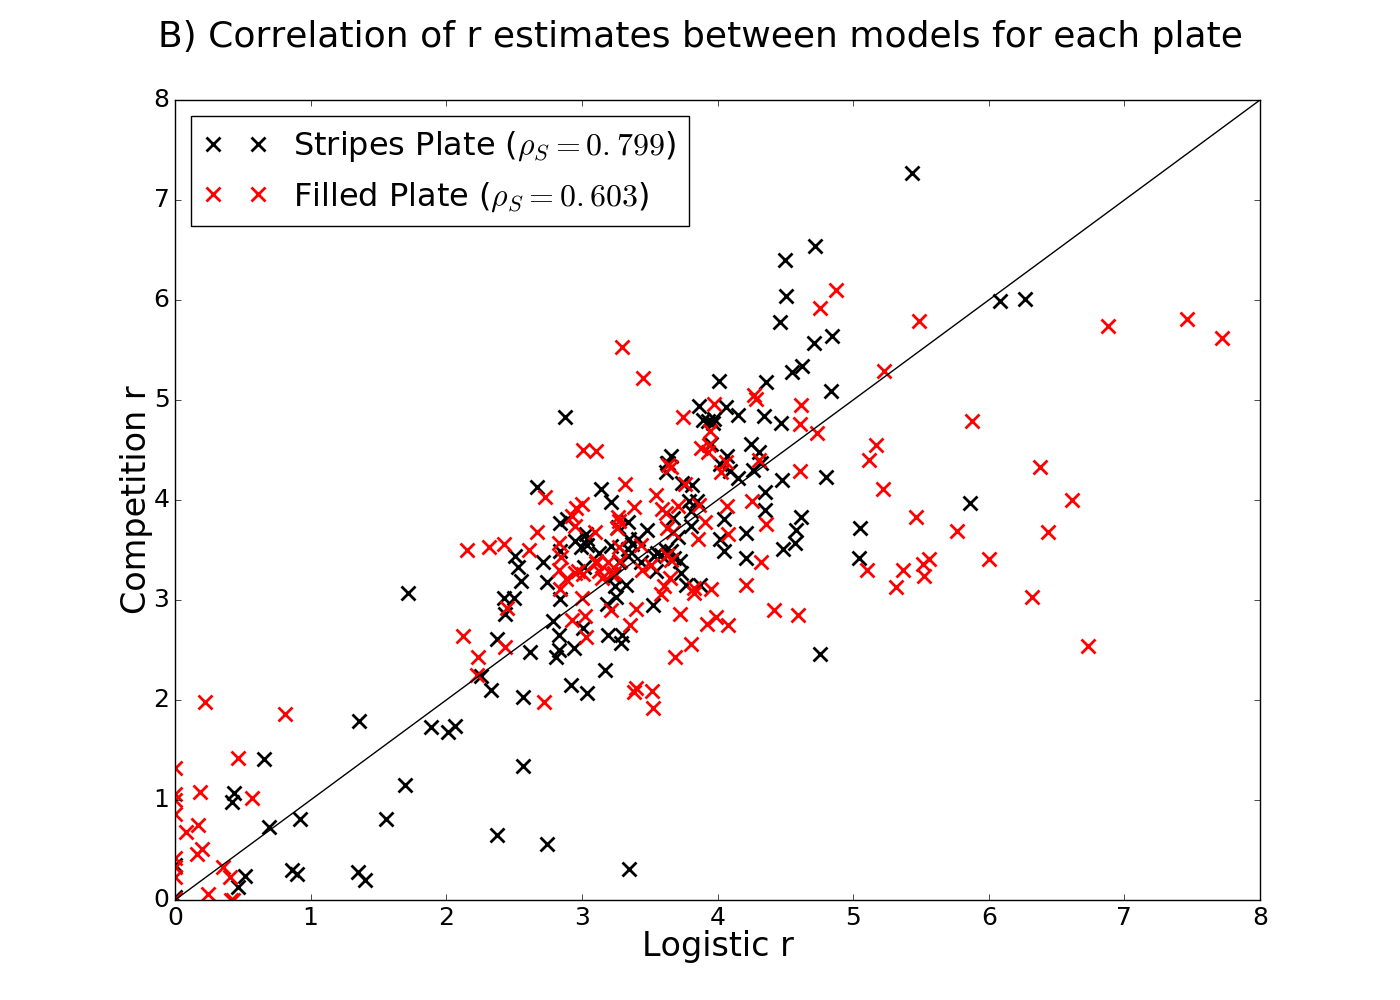
\includegraphics[width=\linewidth]{final/r_correlations_between_models}
%   \captionof{figure}{\textbf{Correlation of r estimates for
%       ``Stripes'' and ``Filled'' plates.}~I fit the competition model
%     and independent model to the ``Stripes'' and ``Filled'' plates in
%     Figure~\ref{fig:stripes_images}. I converted competition model b
%     to logistic model r. I only used data for cultures that were
%     common between the two plates common and removed edge
%     cultures. Pearson correlation coefficients, \(\rho\), are shown in
%     the legends. The line \(y=x\) is also plotted.}
%   \label{fig:r_correlations}
% \end{Figure}

\subsection{Towards a genetic algorithm}

% %\end{multicols}
% \graphicspath{{images/genetic_algorithm/}}
% \begin{Figure}
%   \centering
%   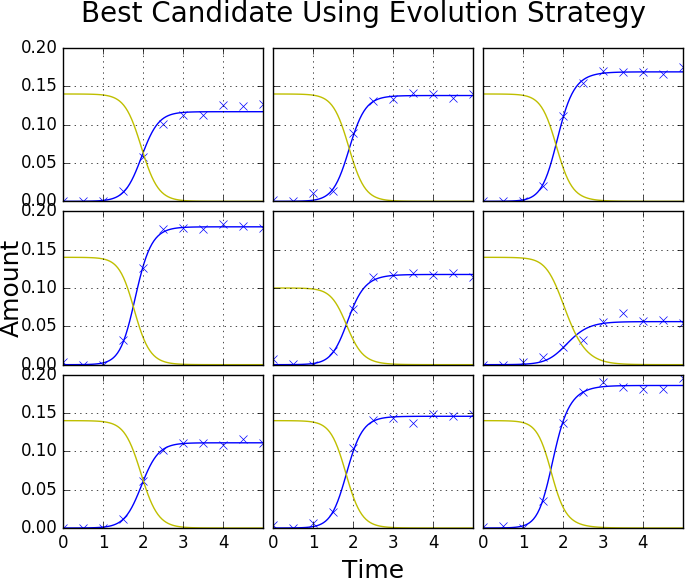
\includegraphics[width=\linewidth]{final/ga_fit_to_sim_true_plate_lvl_trimmed}
%   \captionof{figure}{Genetic algorithm fit to a 3x3 simulation. MIGHT
%     TAKE A LITTLE BIT OF WORK TO REPRODUCE AND COULD USE PARAMETERS
%     FROM THE BEST P15 FIT RATHER THAN JUST PICKING/RANDOMIZING. NEED
%     TO CHECK THAT PLATE LEVEL PARAMETERS WERE ALSO EVOLVED.}
%   \label{fig:3x3_genetic_algorithm_comp_fit_fixed_plate_level}
% \end{Figure}
% %\begin{multicols}{2}
%\end{multicols}
In the interest of developing a quick method for estimating parameters
while avoiding local minima, I investigated how well culture level
parameters can be recovered when plate level parameters are fixed. The
idea is to evolve candidate sets of plate level parameters and
evaluate by fitting data using a gradient method. If culture level
parameters can be recovered reliably, we might not have to worry about
confounding between plate and culture level parameters when evolving
candidates. I took parameter estimates from the five best fits for
P15, and simulated full plate timecoureses at the observed times. I
added a small amount of random noise to imitate real data. I then
fixed plate level parameters to the true values and fit the
competition model just for \(b\). I set bounds of \(0 < b < 200\) and
used 11 evenly spaced guesses of \(b\) in the range
\(\frac{1}{2}\mu_{b} < b < \frac{3}{2}\mu_{b}\) where \(\mu_{b}\) is
the mean true \(b\). These guesses were used in the imaginary
neighbour model to generate 11 sets of initial parameters for the
competition model for each simulation
(Section~\ref{sec:guessing_b}). I solved all models using SciPy's
integrate.odeint, as I had not yet developed code to solve using
libRoadRunner. Otherwise, I fit as for P15
(Section~\ref{sec:fitting_comp}). \(b\) were recovered well even in
the worst instance (Figure~\ref{fig:comp_fit_fixed_plate_level}). In
all instances, estimates were less accurate for slow growing cultures
which are more affected by noise. For some simulations, different
initial parameter sets all achieved a similar quality of fit. For
others, however, certain guesses were much better, suggesting that
multiple fits need to be run for each candidate.

\graphicspath{{images/genetic_algorithm/}}
\begin{Figure}
  \centering
  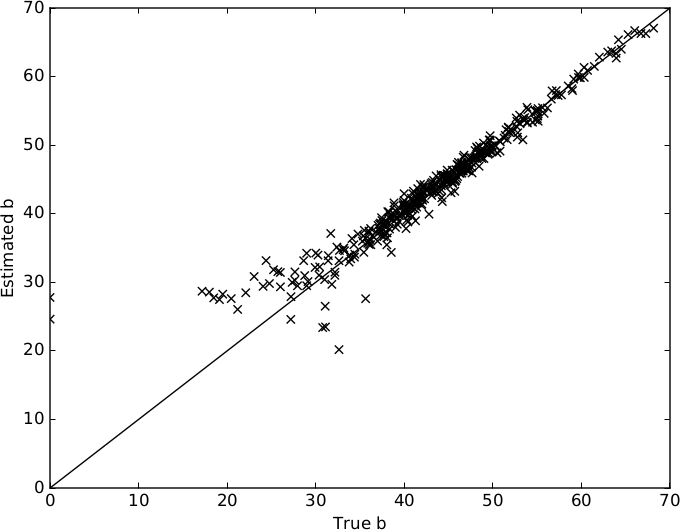
\includegraphics[width=\linewidth]{final/est_b_vs_true_b}
  \captionof{figure}{\textbf{Recovery of true \(b\) values from a
      gradient fit with fixed plate level parameters.} I simulated
    timecourses from the best five competition model fits to p15,
    added a small amount of noise, and used a gradient method to
    recover b given the true plate level parameters. This plot shows
    the worst recovery for the five sets of values.}
  \label{fig:comp_fit_fixed_plate_level}
\end{Figure}

% (Currently only have comp obj funs using different cultures (Stripes
% obj fun 0.66) (Filled obj fun 0.76).)

%%% Local Variables:
%%% mode: latex
%%% TeX-master: "report"
%%% End:
